% Distributed_UAVCtrl_BlockDiagram.tex

\tikzstyle{Block}=[rectangle,draw=blue,rounded corners,line width=0.5mm,
  align=center,minimum height=4em,minimum width=4em]
\tikzstyle{LabelObject}=[fill=white,rectangle,rounded corners,line width=0.5mm,%
	align=center]
\tikzstyle{ArrowObject}=[black,line width=1.0mm, -latex]


\resizebox{!}{0.45\textwidth}{
	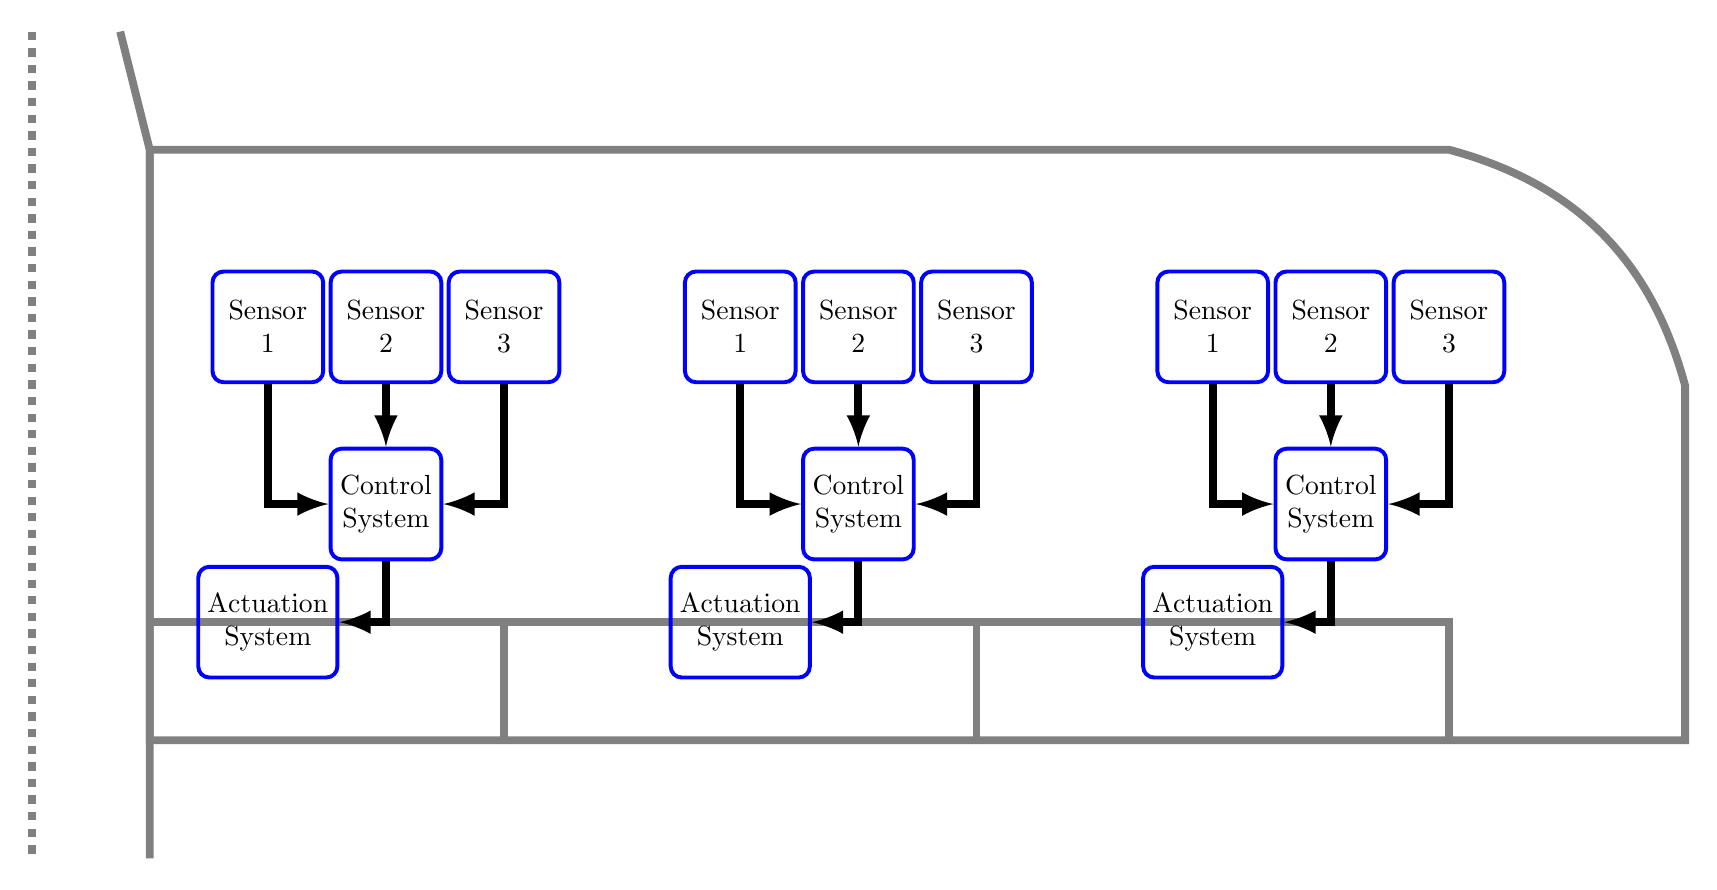
\begin{tikzpicture}[x=1.5cm, y=1.5cm, >=stealth]
		%\draw[help lines,xstep=.5,ystep=.5] (0,1) grid (15,8);
		%\foreach \x in {0,1,...,15} { \node [anchor=north] at (\x/1,0) {0.\x}; }
		%\foreach \y in {1,2,...,8} { \node [anchor=east] at (0,\y/1) {0.\y}; }
		
		% Symmetry Plane
		\draw[dashed,gray,line width=1.0mm] (0.0,8.0) -- (0.0,1.0);
		
		% Fuselage Outline
		\draw[gray,line width=1.0mm] (0.75,8.0) -- (1.0,7.0) -- (1.0,1.0);
		
		% Wing Outline
		\draw[gray,line width=1.0mm] (1.0,7.0) -- (1.0,2.0) -- (14.0,2.0)
		  -- (14.0,5.0) to[bend right] (12.0,7.0) -- cycle;
		% Control Surface 1
		\draw[gray,line width=1.0mm] (4.0,2.0) -- (4.0,3.0) -- (1.0,3.0);
		% Control Surface 2
		\draw[gray,line width=1.0mm] (8.0,2.0) -- (8.0,3.0) -- (4.0,3.0);
		% Control Surface 2
		\draw[gray,line width=1.0mm] (12.0,2.0) -- (12.0,3.0) -- (8.0,3.0);
		
		% Flight control system 1
		\draw(2.0,5.5) node[Block] (SensSystem11) {Sensor\\1};
		\draw(3.0,5.5) node[Block] (SensSystem12) {Sensor\\2};
		\draw(4.0,5.5) node[Block] (SensSystem13) {Sensor\\3};
		\draw(3.0,4.0) node[Block] (CtrlSystem1) {Control\\System};
		\draw(2.0,3.0) node[Block] (ActSystem1) {Actuation\\System};
		% Flight control system 1 arrows
		\draw[ArrowObject] (SensSystem11.south) -- (2,4) -- (CtrlSystem1.west);
		\draw[ArrowObject] (SensSystem12.south) -- (CtrlSystem1.north);
		\draw[ArrowObject] (SensSystem13.south) -- (4,4) -- (CtrlSystem1.east);
		\draw[ArrowObject] (CtrlSystem1.south) -- (3,3) -- (ActSystem1.east);
		
		% Flight control system 2
		\draw(6.0,5.5) node[Block] (SensSystem21) {Sensor\\1};
		\draw(7.0,5.5) node[Block] (SensSystem22) {Sensor\\2};
		\draw(8.0,5.5) node[Block] (SensSystem23) {Sensor\\3};
		\draw(7.0,4.0) node[Block] (CtrlSystem2) {Control\\System};
		\draw(6.0,3.0) node[Block] (ActSystem2) {Actuation\\System};
		% Flight control system 2 arrows
		\draw[ArrowObject] (SensSystem21.south) -- (6,4) -- (CtrlSystem2.west);
		\draw[ArrowObject] (SensSystem22.south) -- (CtrlSystem2.north);
		\draw[ArrowObject] (SensSystem23.south) -- (8,4) -- (CtrlSystem2.east);
		\draw[ArrowObject] (CtrlSystem2.south) -- (7,3) -- (ActSystem2.east);
		
		% Flight control system 3
		\draw(10.0,5.5) node[Block] (SensSystem31) {Sensor\\1};
		\draw(11.0,5.5) node[Block] (SensSystem32) {Sensor\\2};
		\draw(12.0,5.5) node[Block] (SensSystem33) {Sensor\\3};
		\draw(11.0,4.0) node[Block] (CtrlSystem3) {Control\\System};
		\draw(10.0,3.0) node[Block] (ActSystem3) {Actuation\\System};
		% Flight control system 3 arrows
		\draw[ArrowObject] (SensSystem31.south) -- (10,4) -- (CtrlSystem3.west);
		\draw[ArrowObject] (SensSystem32.south) -- (CtrlSystem3.north);
		\draw[ArrowObject] (SensSystem33.south) -- (12,4) -- (CtrlSystem3.east);
		\draw[ArrowObject] (CtrlSystem3.south) -- (11,3) -- (ActSystem3.east);
		
	\end{tikzpicture}
}